% !TeX program = lualatex
% !BIB program = biber
% Lualatex is important to render Fira fonts; with pdflatex it's just the regular one
% ratio 16:9 -- https://tex.stackexchange.com/questions/14336/

% compile two versions, inspired by https://tex.stackexchange.com/a/1501
% use the script "compile-pdf.sh"
\newif\ifhandout
% if flags.tex does not exist, create an empty file to be able to compile in TeXstudio
\input{flags}

\ifhandout
	\documentclass[12pt,aspectratio=169,handout]{beamer}
\else
	\documentclass[12pt,aspectratio=169]{beamer}
\fi

% adjust for 16:9
% https://tex.stackexchange.com/questions/354022/modifying-the-margins-of-all-slides-in-beamer
\setbeamersize{text margin left=0.3cm,text margin right=1.0cm} 

%\usepackage{xcolor}

%%% better TOC
\usetheme[subsectionpage=progressbar]{metropolis}

% name in footer
\setbeamertemplate{frame numbering}{\insertframenumber ~ | Dr.\ Martin Tutek}

% blocks with background globally
\metroset{block=fill}

% adjust the background to be completely white
\setbeamercolor{background canvas}{bg=white}

% typeset mathematics on serif
\usefonttheme[onlymath]{serif}

% better bibliography using biber as backend
\usepackage[natbib=true,backend=biber,style=authoryear-icomp,maxbibnames=30,maxcitenames=2,uniquelist=false,giveninits=true,doi=false,url=false,dashed=false,isbn=false]{biblatex}
% shared bibliography
\addbibresource{../dl4nlp-bibliography.bib}
% disable "ibid" for repeated citations
\boolfalse{citetracker}

\definecolor{76abdf}{RGB}{118, 171, 223}

\setbeamercolor{frametitle}{bg=76abdf, fg=white}

\newcounter{saveenumi}
\newcommand{\seti}{\setcounter{saveenumi}{\value{enumi}}}
\newcommand{\conti}{\setcounter{enumi}{\value{saveenumi}}}

\resetcounteronoverlays{saveenumi}
% \usepackage{movie15}
\usepackage{animate}

\usepackage{xspace}
% Emojis
\usepackage{emoji}
% Figs
\usepackage{graphicx}
\graphicspath{ {./img/} }


% for derivatives, https://tex.stackexchange.com/a/412442
\usepackage{physics}

\usepackage{tikz}
\usetikzlibrary{matrix, positioning}
\usetikzlibrary{angles,quotes} % for angles
\usetikzlibrary{backgrounds} % background
\usetikzlibrary{decorations.pathreplacing} % curly braces
\usetikzlibrary{calligraphy}
\usetikzlibrary{calc} % for neural nets

% for plotting functions
\usepackage{pgfplots}
\usepgfplotslibrary{dateplot}

% sub-figures
\usepackage{caption}
\usepackage{subcaption}

% Checkmark, xmark
\usepackage{pifont}% http://ctan.org/pkg/pifont

% book tabs
\usepackage{booktabs}

% caption*
\usepackage{caption}


% show TOC at every section start
\AtBeginSection{
	\frame{
		\vspace{2em}
		\sectionpage
		\hspace*{2.2em}\begin{minipage}{10cm}
			\tableofcontents[currentsection]
		\end{minipage}
	}
}

% argmin, argmax
\usepackage{amssymb}% http://ctan.org/pkg/amssymb
\usepackage{amsmath}

\DeclareMathOperator*{\argmax}{arg\!\max}
\DeclareMathOperator*{\argmin}{arg\!\min}
% softmax
\DeclareMathOperator*{\softmax}{soft\!\max}
% RNN
\DeclareMathOperator*{\rnn}{RNN}
% RNN star
\DeclareMathOperator*{\rnnstar}{RNN^{*}}
% bi-RNN
\DeclareMathOperator*{\birnn}{biRNN}

% bold math
\usepackage{bm}

% for \mathclap
\usepackage{mathtools}

% algorithms
\usepackage[noend]{algpseudocode}


% for neurons and layers in tikz
\tikzset{
	neuron/.style={draw, rectangle, inner sep=2pt, minimum width=0.75cm, fill=blue!20},
	param/.style={draw, rectangle, inner sep=2pt, minimum width=0.75cm, fill=green!20},
	constant/.style={draw, rectangle, inner sep=2pt, minimum width=0.75cm, fill=black!15},
	state/.style={rectangle, inner sep=2pt, minimum width=0.75cm, fill=black!5},
}

% for strike-through text
\usepackage[normalem]{ulem}


\title{Deep Learning for Natural Language Processing}
\subtitle{Lecture 10 -- Text classification 4:  self-attention and BERT}
\date{June 20, 2023}
\author{Dr.\ Martin Tutek}
\institute{Ubiquitous Knowledge Processing  \hfill 
\includegraphics[height=1.cm]{img/ukp_logo.png} \\
Department of Computer Science\\
Technical University of Darmstadt \hfill \href{https://www.informatik.tu-darmstadt.de/ukp/ukp_home/index.en.jsp}{\underline{UKP Web}}}
%\titlegraphic{\hfill }

\begin{document}

\maketitle

\begin{frame}{Recap}
	In the previous lecture we:
	\begin{itemize}
		\item Introduced the Transformer architecture
		\item Explained what we gain from \textit{contextualized} representations
		\item Analyzed the Transformer attention block
		\item Introduced byte-pair encodings \& what we gain by them
		\item Introduced positional embeddings \& why we need them
	\end{itemize}
\end{frame}


\begin{frame}{Recap: the Transformer architecture}
	\begin{center}
		\begin{figure}[h]
			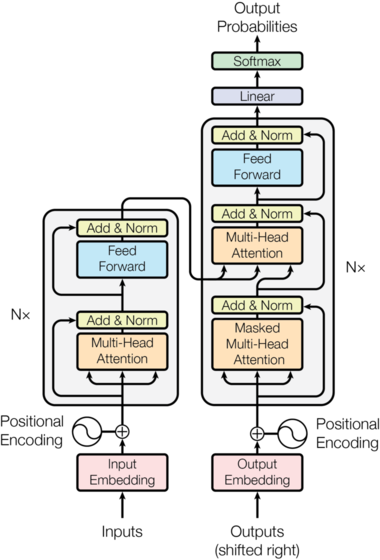
\includegraphics[height=7cm]{anno_transformer}
		\end{figure}
		\end{center}
\end{frame}

\begin{frame}{Recap: Transformer for machine translation}
	We studied the Transformer encoder-decoder for machine translation

	\begin{center}
		\begin{figure}[h]
			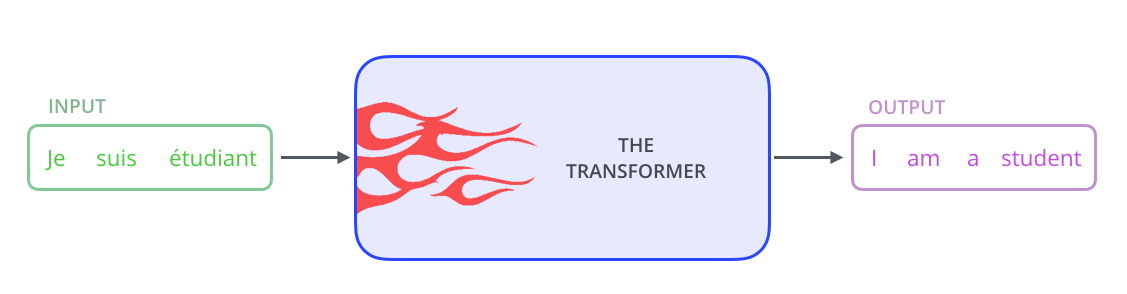
\includegraphics[height=4cm]{the_transformer_mt}
			\caption*{Image source: \href{http://jalammar.github.io/illustrated-transformer/}{\underline{The illustrated Transformer}}}
		\end{figure}
	\end{center}
	\pause
	The model is built of stacked encoder and decoder blocks
\end{frame}


\begin{frame}{Recap: Transformer encoder-decoder}
	\begin{center}
		\begin{figure}[h]
			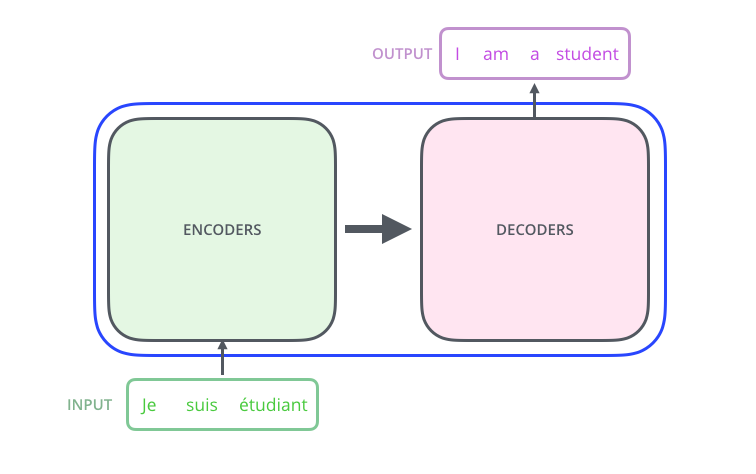
\includegraphics[height=5.7cm]{transformer_encoders_decoders}
			%\caption*{Image source: \href{http://jalammar.github.io/illustrated-transformer/}{\underline{The illustrated Transformer}}}
		\end{figure}
	\end{center}
	\pause
	The encoder and decoder are made of stacked \textbf{encoder} and \textbf{decoder blocks} 
\end{frame}

\begin{frame}{Recap: Transformer encoder-decoder}
	\begin{center}
		\begin{figure}[h]
			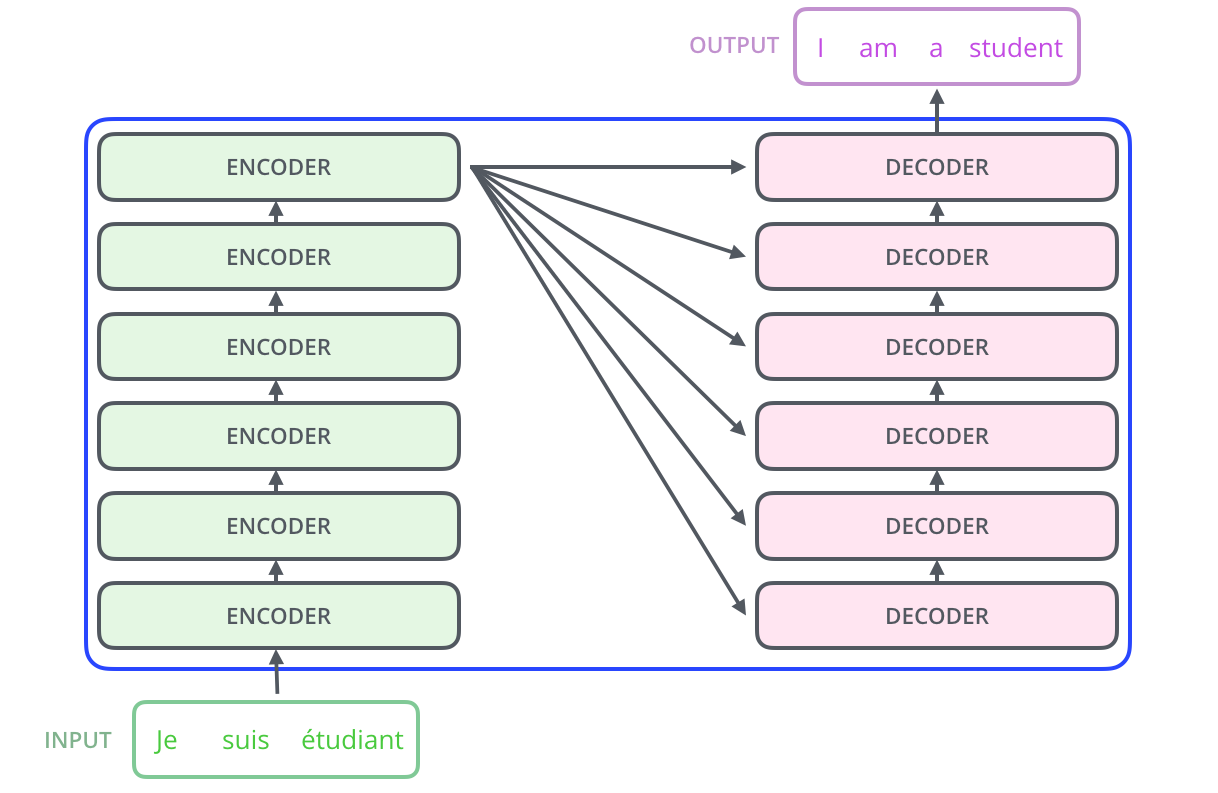
\includegraphics[height=7cm]{transformer_encoder_decoder_stack}
			%\caption*{Image source: \href{http://jalammar.github.io/illustrated-transformer/}{\underline{The illustrated Transformer}}}
		\end{figure}
	\end{center}
\end{frame}


\begin{frame}{Recap: Transformer encoder and decoder block}
	The encoder and decoder blocks are different -- the decoder block has an additional \textbf{encoder-decoder attention} (cross-attention) layer
	\begin{center}
		\begin{figure}[h]
			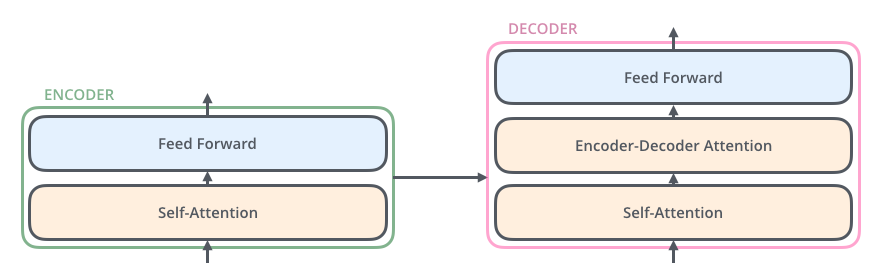
\includegraphics[height=4cm]{transformer_blocks}
			%\caption*{Image source: \href{http://jalammar.github.io/illustrated-transformer/}{\underline{The illustrated Transformer}}}
		\end{figure}
	\end{center}
\end{frame}

\begin{frame}{Recap: Transformer encoder block}
\begin{columns}[T] % align columns
	\begin{column}{.48\textwidth}
	\begin{center}
		\begin{figure}[h]
			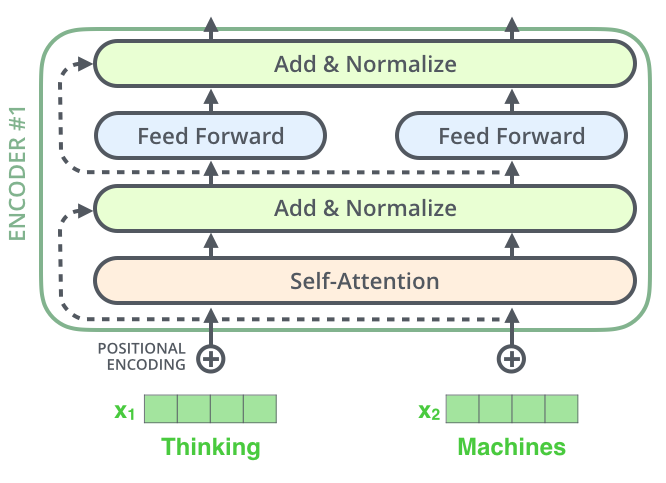
\includegraphics[height=5.5cm]{transformer_residual_layer_norm}
			%\caption*{Image source: \href{http://jalammar.github.io/illustrated-transformer/}{\underline{The illustrated Transformer}}}
		\end{figure}
	\end{center}
\end{column}

\begin{column}{.48\textwidth}
	Each Transformer encoder block consists of:
	\begin{enumerate}
		\item Self-attention: \textbf{contextualize} representations
		\item \textbf{Residual} connection + \textbf{normalization}
		\item \textbf{Feed-forward} layer ($1$ hidden layer NN)
		\item \textbf{Residual} connection + \textbf{normalization}
	\end{enumerate}
\end{column}
\end{columns}
\end{frame}

\begin{frame}{Recap: Transformer encoder-decoder}
	\begin{center}
		\begin{figure}[h]
			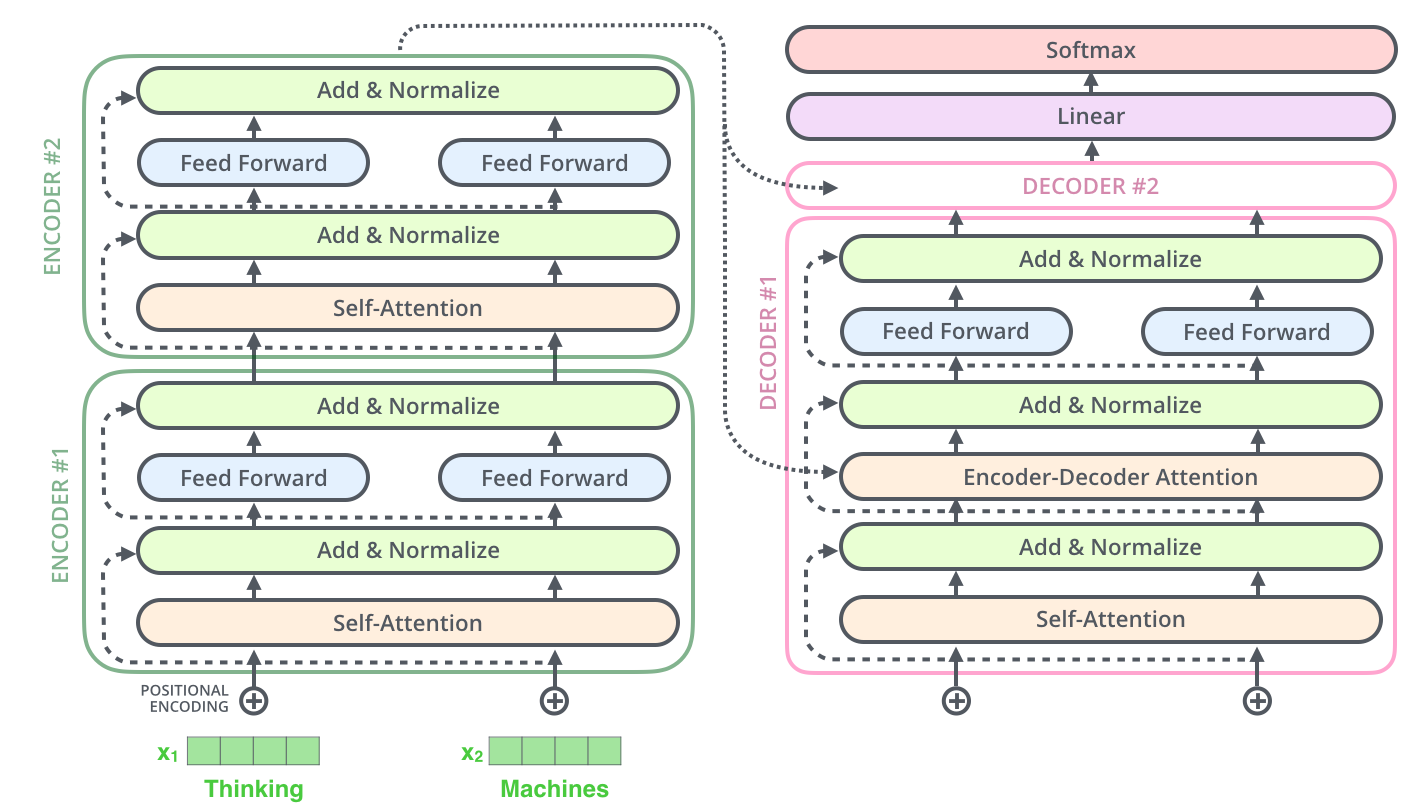
\includegraphics[height=7cm]{transformer_encoder_decoder_stack_full}
			%\caption*{Image source: \href{http://jalammar.github.io/illustrated-transformer/}{\underline{The illustrated Transformer}}}
		\end{figure}
	\end{center}
\end{frame}

\begin{frame}{Recap: Transformer decoding in practice}
	\begin{center}
		\huge{Transformer decoding gif}
	\end{center}
	% \animategraphics[autoplay,loop,controls,height=7cm]{10}{gifs/transformer-decoding-frames/frame_}{000}{157}
\end{frame}



%\begin{frame}{Recap contents}
%	\begin{itemize}
%		\item MHA
%		\item BPE 
%		\item Positional encodings
%	\end{itemize}
%\end{frame}

\section{Next steps?}

\begin{frame}{Motivation}
	The transformer encoder-decoder model is \textbf{really} good at sequence-to-sequence tasks
	\pause
	\begin{itemize}
		\item It \textbf{scales} well (to many layers \& parameters)
		\pause
		\item It \textbf{performs} well on long sequences
		\pause
		\item It's \textbf{easier to optimize} (residual connections)
		\pause
		\item It's \textbf{faster to run} (parallel processing in encoder)
	\end{itemize}
	\pause
	\vspace{1em}
	However -- we can \textbf{only} use it for the \textbf{task it was trained on}
\end{frame}

\begin{frame}{Motivation}

	\begin{block}{Transfer learning}
		... is applying knowledge gained when \textbf{solving one task} to a \textbf{related} task.

		Gained knowledge $\to$ encoded in a \textbf{trained model}.
	\end{block}

	\pause

	\vspace{1em}
	Where have we seen something like this before?
	\pause
	\begin{itemize}
		\item \textbf{Word2vec} (CBOW \& Skip-gram)
	\end{itemize}
	\pause
	We \textbf{train} the word embeddings on an \textit{auxiliary task}, then use them as input for other models
	\pause
	Can we apply this to \textbf{Transformer} encoders to obtain pretrained \textbf{contextualized} embeddings?

\end{frame}

\section{BERT}

\begin{frame}{BERT}

\begin{center}
	\begin{figure}[h]
		
\includegraphics[height=4cm]{bert-google}
	\end{figure}

	\begin{figure}[h]
		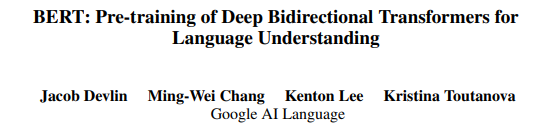
\includegraphics[height=2cm]{bert-paper}
	\end{figure}
\end{center}

\end{frame}


\begin{frame}{BERT}

	What \textbf{we have}
	\begin{itemize}
		\item A model: the Transformer
	\end{itemize}

	\pause
	What \textbf{we want}
	\begin{itemize}
		\item Pretrained \textit{contextualized} word representations
	\end{itemize}

	\pause
	What \textbf{we need}
	\begin{itemize}
		\item The \textbf{auxiliary pretraining task}
		\pause
		\item ... ideally, it should not require labeled data (expensive)
	\end{itemize}

\end{frame}

\begin{frame}{BERT: pretraining objective}

	\textbf{Recall}: what was the word2vec training objective?
	\pause
	\begin{itemize}
		\item \textbf{CBOW}: predict \textbf{center word} given \textbf{context words}
		\pause
		\begin{figure}[h]
			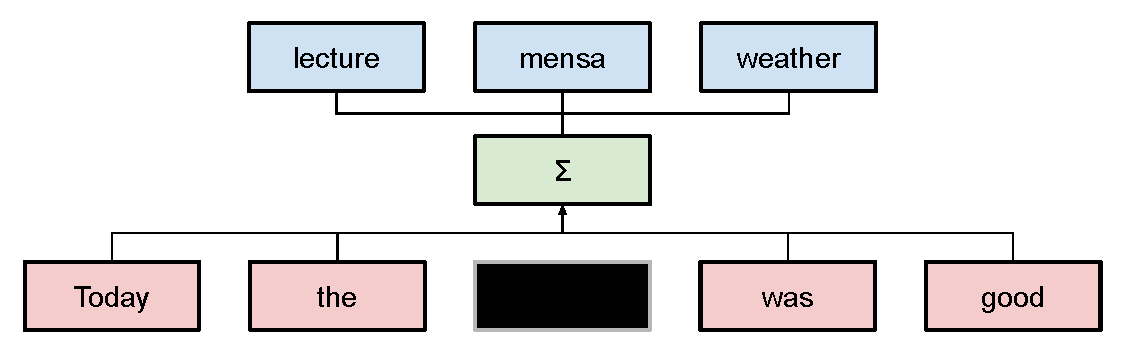
\includegraphics[height=3cm]{word2vec_cbow.pdf}
		\end{figure}
		\pause
		\item \textbf{Skip-gram}: predict \textbf{context words} given \textbf{center word}
	\end{itemize}
	\pause
	Can we use a \textbf{similar} task with Transformer models?
\end{frame}

\begin{frame}{BERT: pretraining objective}

	\begin{figure}[h]
		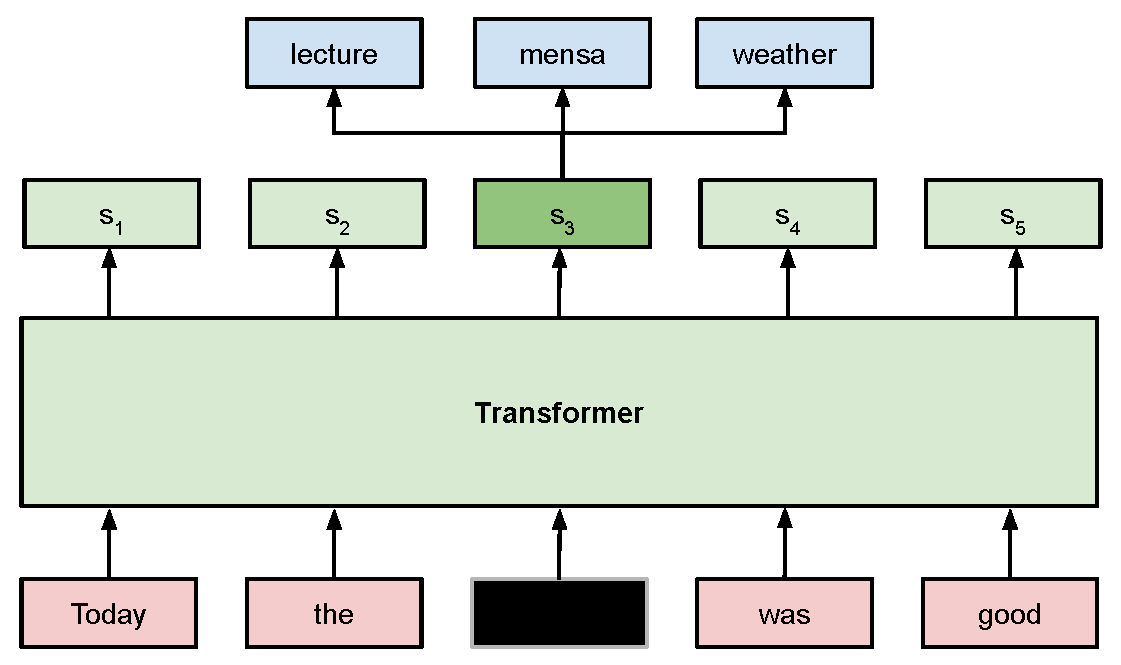
\includegraphics[height=6.5cm]{bert_modeling.pdf}
	\end{figure}

\end{frame}

\begin{frame}{BERT: pretraining objective}
\begin{columns}[T] % align columns
	\begin{column}{.58\textwidth}
	\begin{figure}[h]
		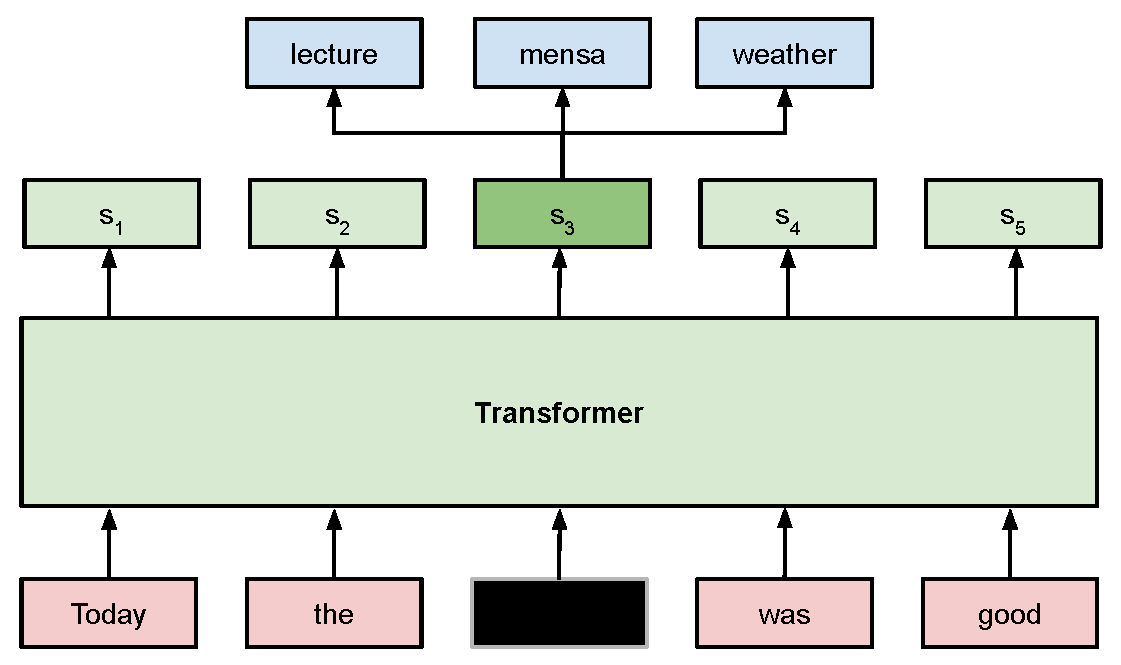
\includegraphics[height=5cm]{bert_modeling.pdf}
	\end{figure}
	\end{column}

	\begin{column}{.38\textwidth}
		\begin{enumerate}
		\item For an input sequence $\{\bm{x}_i\}_{i=1}^n$, we \textbf{mask} an input token(s)
		\pause
		\item We encode the inputs with a Transformer \textbf{encoder}
		\pause
		\item We \textbf{reconstruct} the masked token(s)
		\end{enumerate}
		\pause 
		What is \textit{masking}?
	\end{column}
\end{columns}

\end{frame}

\begin{frame}[fragile]{BERT: masked language modeling (MLM)}

The \textbf{Transformer} model contextualizes an input sequence $\{\bm{x}_i\}_{i=1}^n$ of (subword) tokens into a sequence of hidden states $\{\bm{s}_i\}_{i=1}^n$.

\pause

\begin{enumerate}
	\item With probability $p_{mlm}$, mask \textbf{each input token} ($p_{mlm}=0.15$)
	\pause
	\item \textbf{If} a token is masked
	\begin{itemize}
		\item $80\%$ of the time, replace it with a special \verb|<MASK>| token
		\pause
		\item $10\%$ of the time, replace it with a \textbf{random} token
		\pause
		\item $10\%$ of the time, \textbf{do not mask it}
	\end{itemize}
	\pause
	\item \textbf{Only} for the \textbf{masked tokens}
	\begin{itemize}
		\item Predict which token was masked
	\end{itemize}
\end{enumerate}

\end{frame}

\begin{frame}{BERT:  masked language modeling (MLM) \href{http://jalammar.github.io/illustrated-bert/}{[\underline{Image source}]}}

	\begin{figure}[h]
		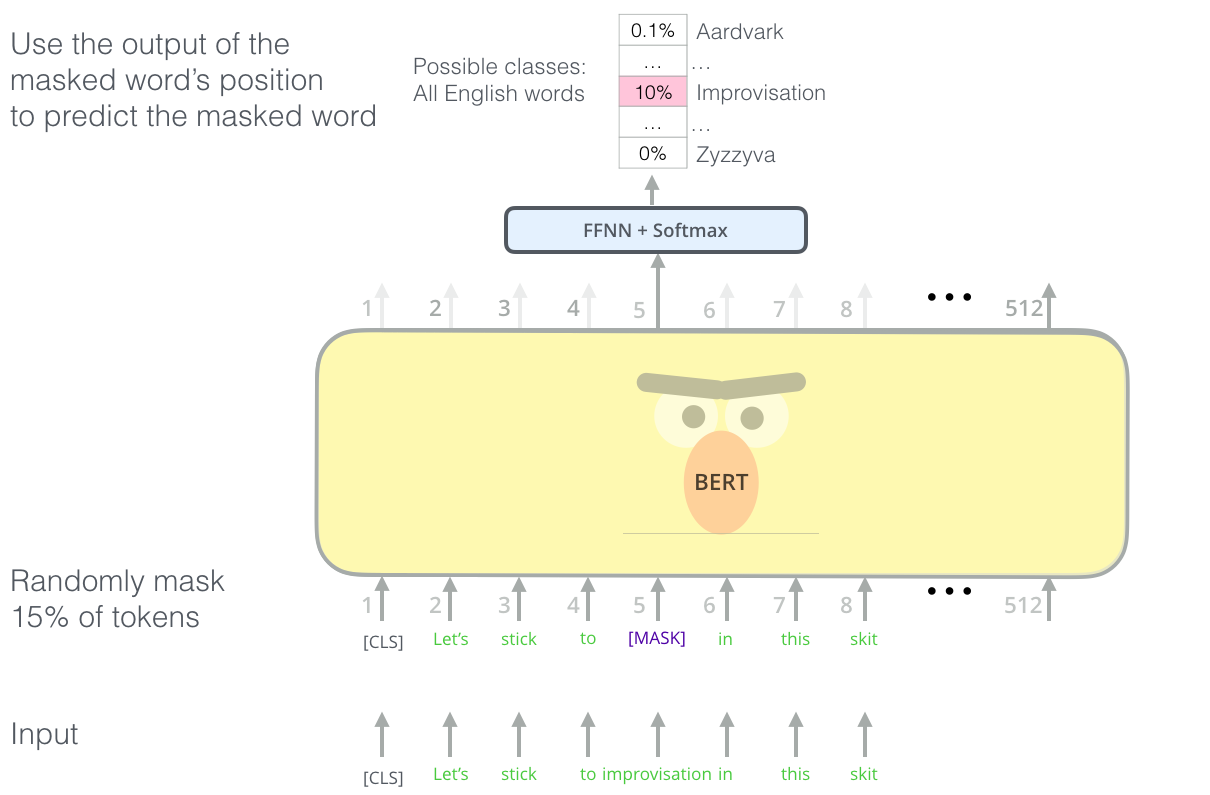
\includegraphics[height=7.5cm]{BERT-language-modeling-masked-lm.png}
		%\caption*{Image from \href{http://jalammar.github.io/illustrated-bert/}{\underline{The illustrated BERT}}}
	\end{figure}

\end{frame}



\begin{frame}{BERT: masked language modeling (MLM)}
	And... it works

	\begin{figure}[h]
		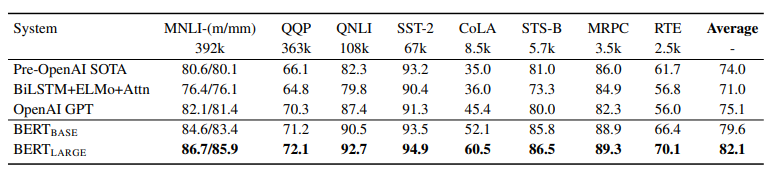
\includegraphics[height=3.25cm]{bert-results}
		\caption*{GLUE Test results (\href{https://gluebenchmark.com/leaderboard}{\underline{GLUE benchmark}}). Table from \href{https://arxiv.org/pdf/1810.04805.pdf}{\underline{BERT paper}}}
	\end{figure}
	\pause
	However -- we are \textit{not there yet}
	\pause
	\begin{itemize}
		\item How do we obtain \textbf{sentence representations}?
	\end{itemize}

\end{frame}

\begin{frame}[fragile]{BERT: next sentence prediction (NSP)}

	\begin{columns}[T] % align columns
		\begin{column}{.48\textwidth}
		\begin{figure}[h]
			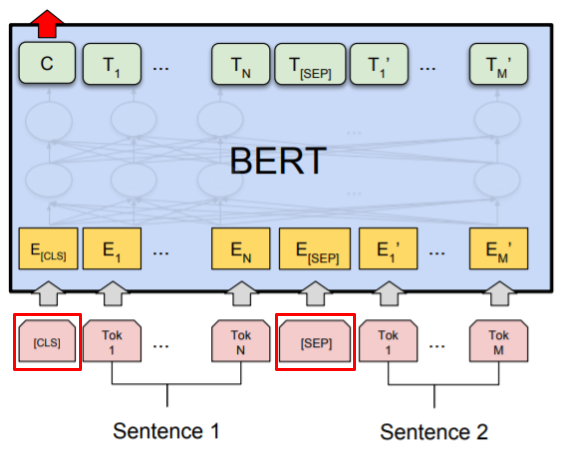
\includegraphics[height=5cm]{bert_nsp_anno.png}
		\end{figure}
		\end{column}
	
		\begin{column}{.48\textwidth}
			We want to have a sentence representation \textbf{out-of-the-box}
			\pause
			\begin{enumerate}
				\item We add a special \verb|CLS| token as the \textbf{sentence representation}
				\item We add a special \verb|SEP| token to separate \textbf{two input sentences}
				\pause
				\item We predict (based on the \verb|CLS| token) if Sent.$1$ \textbf{directly precedes} Sent.$2$ in the pretraining dataset 
			\end{enumerate}

		\end{column}
	\end{columns}
\end{frame}

\begin{frame}{BERT: next sentence prediction (NSP)\href{http://jalammar.github.io/illustrated-bert/}{[\underline{Image source}]}}

	\begin{figure}[h]
		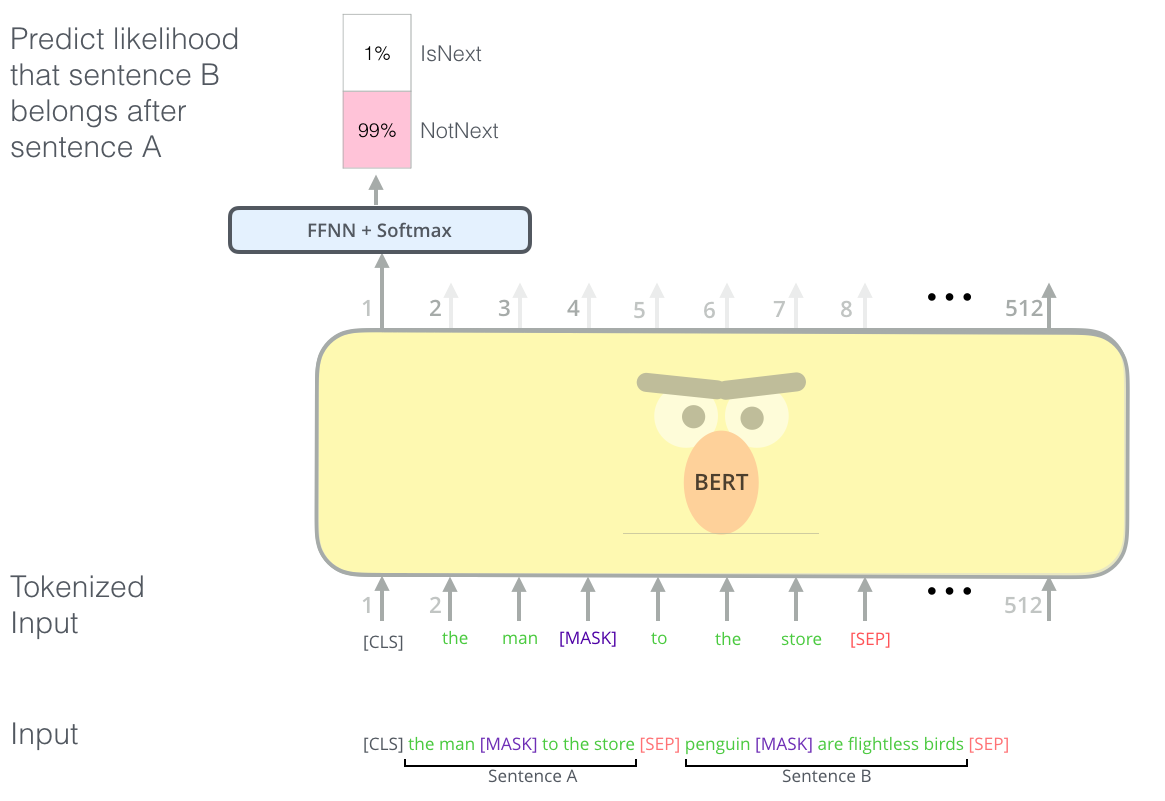
\includegraphics[height=7.5cm]{bert-next-sentence-prediction.png}
		%\caption*{Image from \href{http://jalammar.github.io/illustrated-bert/}{\underline{The illustrated BERT}}}
	\end{figure}

\end{frame}

\begin{frame}{BERT: pretraining}

Combining the \textbf{MLM} and \textbf{NSP} objectives:

\begin{enumerate}
	\item Take a \textbf{large corpus} of unstructured text (Wikipedia, BookCorpus) and retain information about position of \textbf{sentences} in each article
	\pause
	\item Create the input sequence: $\mathbf{in} = \text{[CLS]} \{\bm{x}^1_{i}\}_{i=1}^{n_1} \text{[SEP]} \{\bm{x}^2_{i}\}_{i=1}^{n_2}$
	\pause
	\begin{enumerate}
	\item Sample Sentence\_$1$ from the dataset
	\pause
	\item With $p_{nsp} = 0.5$, take Sentence\_$2$ as the following sentence (heads) \textbf{or} randomly sample it (tails) 
	\end{enumerate}
	\pause
	\item Mask $p_{mlm}=0.15$ of \textbf{non-special} input tokens (recall: $80/10/10$)
	\pause
	\item Encode inputs with transformer encoder: $ \mathbf{trf}(\mathbf{in}) \to \{ \bm{s}_{i}\}_{i=1}^{n_1 + n_2 + 2} $
	\pause
	\item Pretraining tasks
	\begin{enumerate}
	\item \textbf{MLM}: reconstruct masked tokens $\bm{s}_i \to \bm{x}_i \quad \forall i \in  \{\text{masked}\}$;
	\item \textbf{NSP}: predict if sentences are successors $\bm{s}_1 \to \{0,1\}$.
	\end{enumerate}
\end{enumerate}

\end{frame}
	
\begin{frame}{BERT: summary}

BERT is a \textbf{pretrained language model (PLM)}

\pause

\begin{itemize}
	\item Through a language modeling pretraining task, the model has learned to recognize \textbf{patterns of language} and apply them for the task of \textbf{text reconstruction}
	\pause
	\item Text reconstruction is, however, \textbf{rarely useful} in isolation
	\pause
	\item In practice: use the PLM as a \textbf{starting point} (a very good initialization) for \textbf{fine-tuning} (additional training) for another task
\end{itemize}

\end{frame}

\begin{frame}{BERT: applications}

Now we have the pretrained BERT -- a Transformer encoder.

\begin{figure}[h]
	
\includegraphics[height=3.5cm]{bert-viz}
\end{figure}

\pause
What's next?
\pause

\begin{itemize}
	\item How to use this model for \textbf{downstream tasks}?
\end{itemize}
\end{frame}

\subsection{Fine-tuning BERT}

\begin{frame}{Using BERT for NLP tasks}

	\textbf{Fine-tuning} is the procedure where we start from a base \textbf{pretrained} model and adapt its internal representations to our task.

	\pause

	Fine-tuning variants:
	\begin{enumerate}
		\item \textbf{Vanilla fine-tuning}: add a \textbf{decoder head} to the model, then:
		\pause
		\begin{enumerate}
			\pause
			\item Train \textbf{only} the decoder head;
			\pause
			\item Train \textbf{progressively} more layers: first the decoder head, then also the last layer, then also the second to last ...;
			\pause
			\item Train the \textbf{entire network} at the same time, maybe with \textbf{different learning rates} per layer.
		\end{enumerate} 
		\pause
		\item \textbf{Adapters}: additional randomly initialized layers inserted inside the transformer layers
		\pause
		\item \textbf{Prompting} \& \textbf{in-context learning}: future lectures
	\end{enumerate}

\end{frame}

\begin{frame}{Using BERT for NLP tasks}

What exactly are \textbf{decoder heads}?
\pause
\vspace{1em}

\textbf{Randomly initialized} additional layers (usually linear) added \textbf{on top} of the pretrained model which \textbf{perform the downstream task}.

\pause

\begin{figure}[h]
	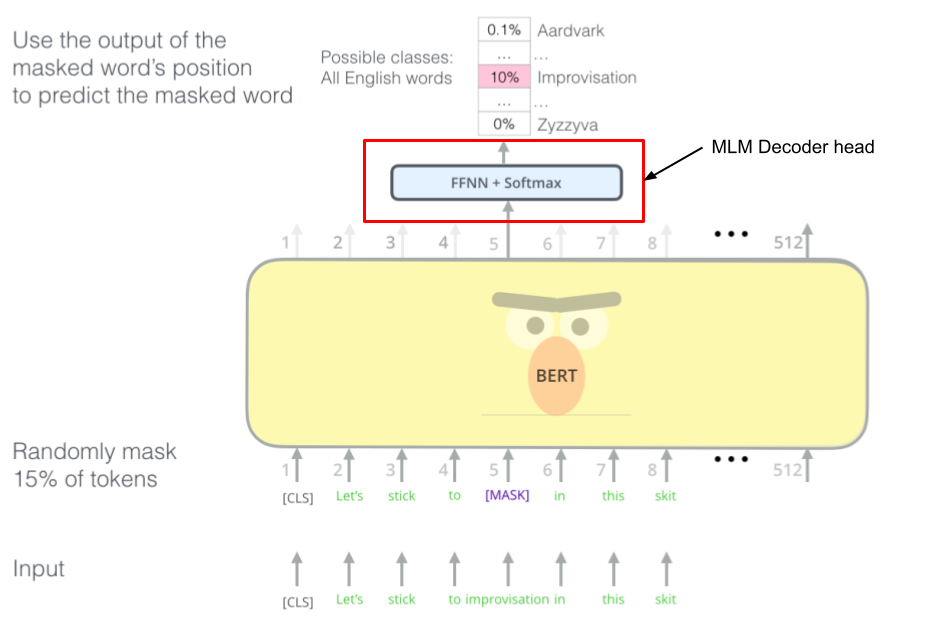
\includegraphics[height=4.5cm]{bert-decoder-head-hl}
\end{figure}

\end{frame}


\begin{frame}{Using BERT: single sequence classification}
	\begin{columns}[T] % align columns
		\begin{column}{.48\textwidth}
		\begin{figure}[h]
			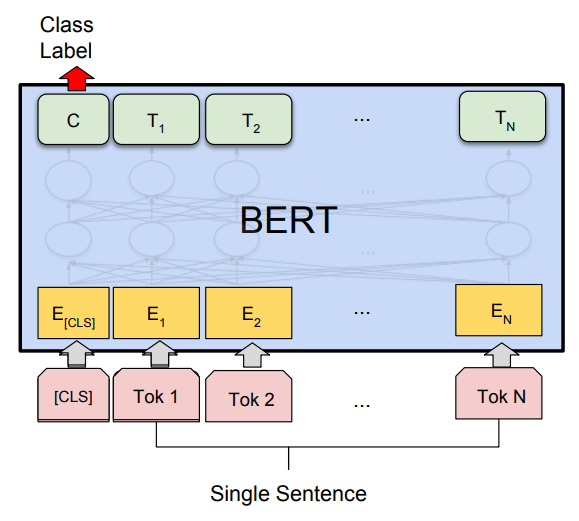
\includegraphics[height=5.5cm]{bert-single-sentence-clf}
			\caption*{Image from \href{https://arxiv.org/pdf/1810.04805.pdf}{\underline{BERT paper}}}
		\end{figure}
	\end{column}
	
	\begin{column}{.48\textwidth}
		For single \textbf{sequence} classification:
		\begin{enumerate}
			\item Add a randomly initialized \textbf{task decoder head} to the model
			\pause
			\item \textbf{Encode} the sequence along with the [CLS] special token
			\pause
			\item Use the \textbf{[CLS]} representation as input to decoder head
		\end{enumerate}
		\pause
		Alternatives to using CLS?
		\begin{itemize}
			\item Averaging over \textbf{token representations}
			\pause
			\item ... from the \textbf{last four layers}
		\end{itemize}
	\end{column}
\end{columns}
\end{frame}


\begin{frame}{Using BERT: sentence pair classification}
	\begin{columns}[T] % align columns
		\begin{column}{.48\textwidth}
	\begin{figure}[h]
		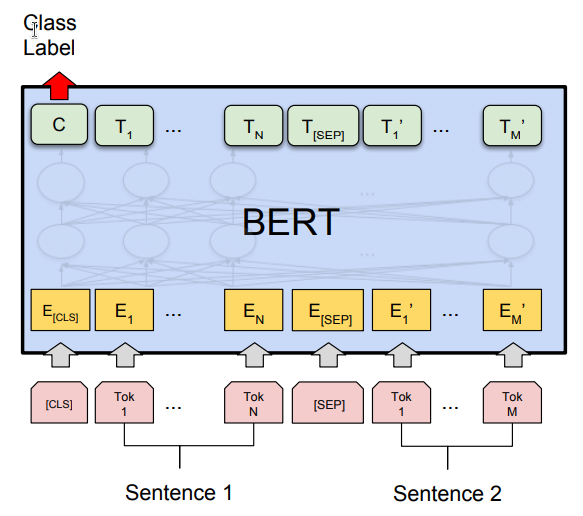
\includegraphics[height=5.5cm]{bert-pair-classification}
		\caption*{Image from \href{https://arxiv.org/pdf/1810.04805.pdf}{\underline{BERT paper}}}
	\end{figure}
\end{column}

\begin{column}{.48\textwidth}
	For \textbf{pair sequence} classification:
	\begin{enumerate}
		\item Add a randomly initialized \textbf{task decoder head} to the model
		\pause
		\item \textbf{Encode} \textbf{both sequences} along with the [CLS] special token
		\pause
		\item Use the \textbf{[CLS]} token representation as input to decoder head
	\end{enumerate}
\end{column}

\end{columns}
\end{frame}

\begin{frame}{Using BERT: span extraction QA}
	\begin{columns}[T] % align columns
		\begin{column}{.48\textwidth}
	\begin{figure}[h]
		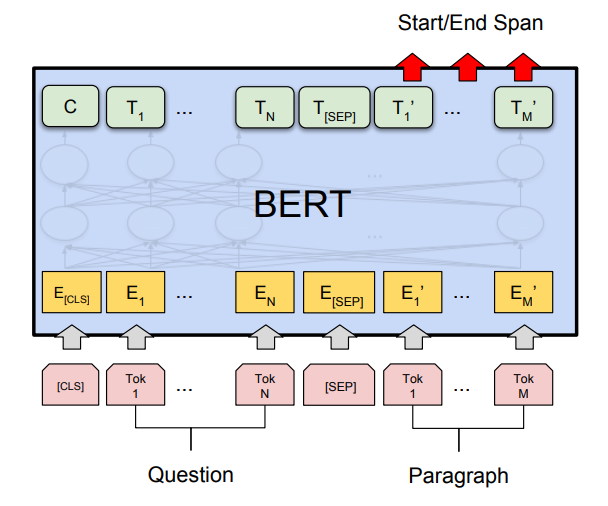
\includegraphics[height=5.5cm]{bert-spanex-qa}
		\caption*{Image from \href{https://arxiv.org/pdf/1810.04805.pdf}{\underline{BERT paper}}}
	\end{figure}
\end{column}

\begin{column}{.48\textwidth}
	For \textbf{span extraction} QA:
	\begin{enumerate}
		\item Add randomly initialized \textbf{start-of-span} and \textbf{end-of-span} \textbf{vectors} to the model.
		\pause
		\item \textbf{Encode} \textbf{both sequences}
		\pause
		\item Highest dot product of \textbf{token representation} with start-of-span and end-of-span is the predicted span
		\pause
		\begin{itemize}
			\item ... such that end-of-span $>$ start-of-span
		\end{itemize}
	\end{enumerate}
\end{column}
\end{columns}

\end{frame}

\begin{frame}{Using BERT: sequence labeling}
	\begin{columns}[T] % align columns
		\begin{column}{.48\textwidth}
	\begin{figure}[h]
		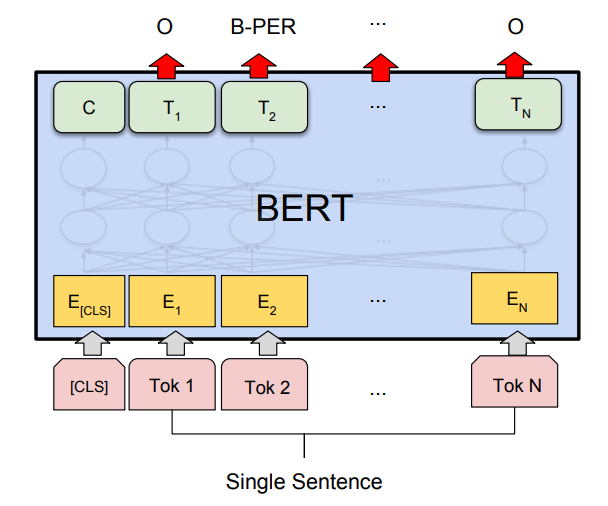
\includegraphics[height=5.5cm]{bert-seq-labeling}
		\caption*{Image from \href{https://arxiv.org/pdf/1810.04805.pdf}{\underline{BERT paper}}}
	\end{figure}
\end{column}

\begin{column}{.48\textwidth}
	For \textbf{sequence labeling}:
	\begin{enumerate}
		\item Add a randomly initialized \textbf{task decoder head} to the model
		\pause
		\item \textbf{Encode} the sequence along with the [CLS] special token
		\pause
		\item Use the \textbf{token representations} as inputs to decoder head
	\end{enumerate}
\end{column}
\end{columns}

\end{frame}


\subsection{Variants of pretraining tasks}

\begin{frame}{Variants of pretraining tasks}

We have used \textbf{MLM} and \textbf{NSP} -- are there some \textit{better} tasks for pretraining language models?
\pause

Perhaps in an \textbf{encoder-decoder} setup?

\pause

\begin{figure}[h]
	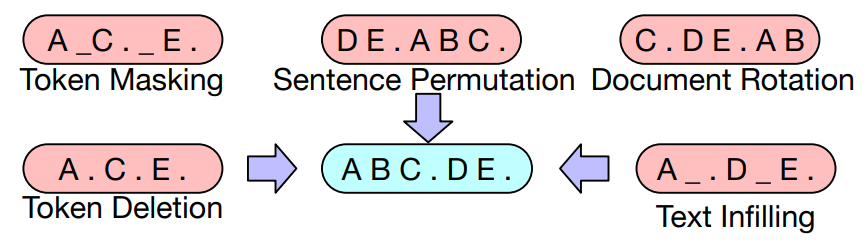
\includegraphics[height=3.5cm]{bart-pretraining-tasks}
	\caption*{Image from \href{https://arxiv.org/pdf/1910.13461.pdf}{\underline{BART paper}}}
\end{figure}

\end{frame}

\begin{frame}{Variants of pretraining tasks}

	\begin{itemize}
		\item \textbf{Language modeling}
		\pause
		\item \textbf{Token masking}: MLM
		\pause
		\item \textbf{Token deletion}: masking, but \textbf{completely removes tokens} from input -- model needs to determine where a token is missing
		\pause 
		\item \textbf{Text infilling}: masking, but \textbf{multiple} tokens are replaced with a \textbf{single} [MASK] token at the same time
		\pause
		\item \textbf{Sentence permutation}: input \textbf{permuted sentence}, reconstruct correct word order (\textit{linearization})
		\pause
		\item \textbf{Document rotation}: document is rotated so that it starts from a \textbf{random token}. The model has to determine the actual start of the document.
	\end{itemize}
	
\end{frame}

\begin{frame}{Variants of (supervised) pretraining tasks}

What if we decide to use \textbf{supervised data} -- but from various datasets?

\pause

\begin{figure}[h]
	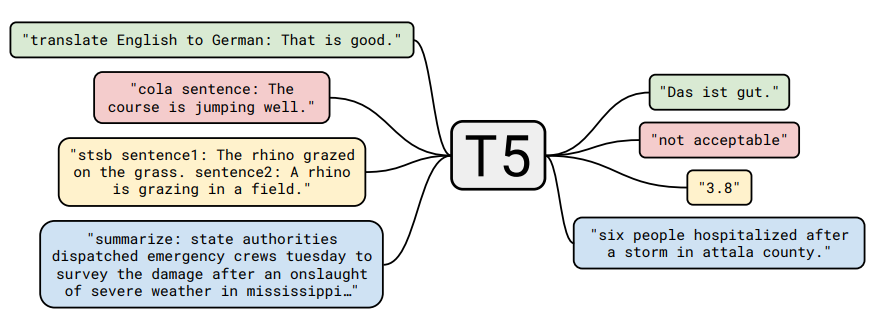
\includegraphics[height=4.5cm]{t5-objectives}
	\caption*{Image from \href{https://jmlr.org/papers/volume21/20-074/20-074.pdf}{\underline{T5 paper}}}
\end{figure}

\end{frame}


\begin{frame}{Pretrained language model architectures}
	\begin{figure}[h]
		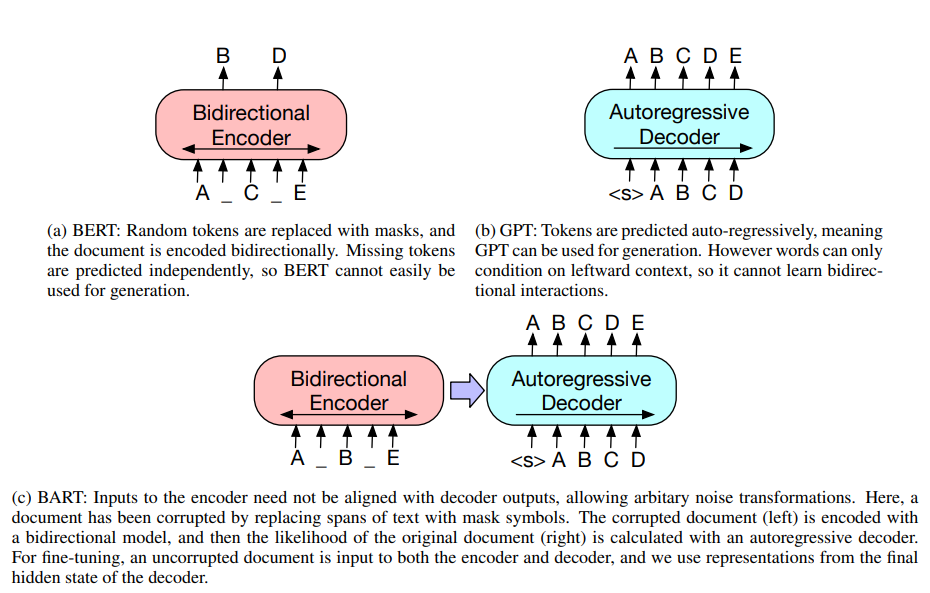
\includegraphics[height=6.5cm]{pretrained-lm-variants}
		\caption*{Image from \href{https://arxiv.org/pdf/1910.13461.pdf}{\underline{BART paper}}}
	\end{figure}
	
\end{frame}

% \subsection{Other pretrained language models}
% Lecture 11

\begin{frame}{Takeaways}
	
\begin{itemize}
	\item BERT is a pretrained language model which produces \textbf{contextualized} token representations of input TeXstudio
	\item It can be used as an \textbf{initialization} (starting point) for \textbf{fine-tuning} task-specific models
	\begin{itemize}
		\item Extras: [CLS] and [SEP] tokens
		\item Applications of BERT in classification, sequence labeling and span-extraction QA
	\end{itemize} 
	\item Other pretraining tasks are also viable
	\begin{itemize}
		\item \textbf{Unsupervised}: sentence permutation, text infilling
		\item \textbf{Supervised}: translation, summarization
	\end{itemize}
\end{itemize}
	
\end{frame}

\begin{frame}{Useful resources}
	
	\begin{itemize}
		\item \href{https://nlp.seas.harvard.edu/2018/04/03/attention.html}{\underline{The annotated Transformer}} by Sasha Rush
		\item \href{http://jalammar.github.io/illustrated-transformer/}{\underline{The illustrated Transformer}} by Jay Allamar
		\item \href{http://jalammar.github.io/illustrated-bert/}{\underline{The illustrated BERT}} by Jay Allamar
	\end{itemize}
		
	\end{frame}
	


\begin{frame}{License and credits}

	\begin{columns}
		\begin{column}{0.7\textwidth}
			Licensed under Creative Commons Attribution-ShareAlike 4.0 International (CC BY-SA 4.0)
		\end{column}
		\begin{column}{0.2\textwidth}
			
\includegraphics[width=0.9\linewidth]{img/cc-by-sa-icon.pdf}
		\end{column}
	\end{columns}
	
	\bigskip
	
	Credits
	
	\begin{scriptsize}
		
		Martin Tutek
		
		Content from ACL Anthology papers licensed under CC-BY \url{https://www.aclweb.org/anthology}
		
	
	\end{scriptsize}
	
\end{frame}



\end{document}

